\documentclass[aspectratio=169]{beamer}
\usepackage{luatexja}
\usepackage{jslogo}
\usepackage[hiragino-pro,deluxe]{luatexja-preset}

\usetheme{EastLansing}
\renewcommand{\kanjifamilydefault}{\gtdefault}
\setbeamertemplate{navigation symbols}{}
\setbeamerfont{title}{family=\gtfamily} % ゴシック
\setbeamerfont{author}{family=\gtfamily} % ゴシック
\setbeamerfont{frame}{family=\gtfamily} % ゴシック
\setbeamerfont{frametitle}{family=\mgfamily} % 丸ゴシック
\setbeamertemplate{blocks}[rounded]

\title{\LaTeX 処理自動化ツールClut\TeX の紹介}
\author{荒田 実樹}
\date{2018年10月11日}

\begin{document}
\begin{frame}\frametitle{}
  \titlepage
\end{frame}
\begin{frame}\frametitle{\LaTeX 処理}
  みなさん、\LaTeX{}文書はどうやって処理していますか?
  \pause
  \begin{enumerate}
    %\renewcommand{\labelenumi}{\Alph{\theenumi}}
  \item コマンドラインで\texttt{platex}/\texttt{dvipdfmx}等のコマンドを直接叩いている
  \item \texttt{latexmk}等の処理自動化ツールを使っている
  \item \TeX{}worksや\TeX{}Shop等の統合環境を使っている
  \item OverleafやCloud LaTeX等のクラウド環境を使っている
  \end{enumerate}
\end{frame}
\begin{frame}[plain]
  \begin{block}{処理前}
    \centering
    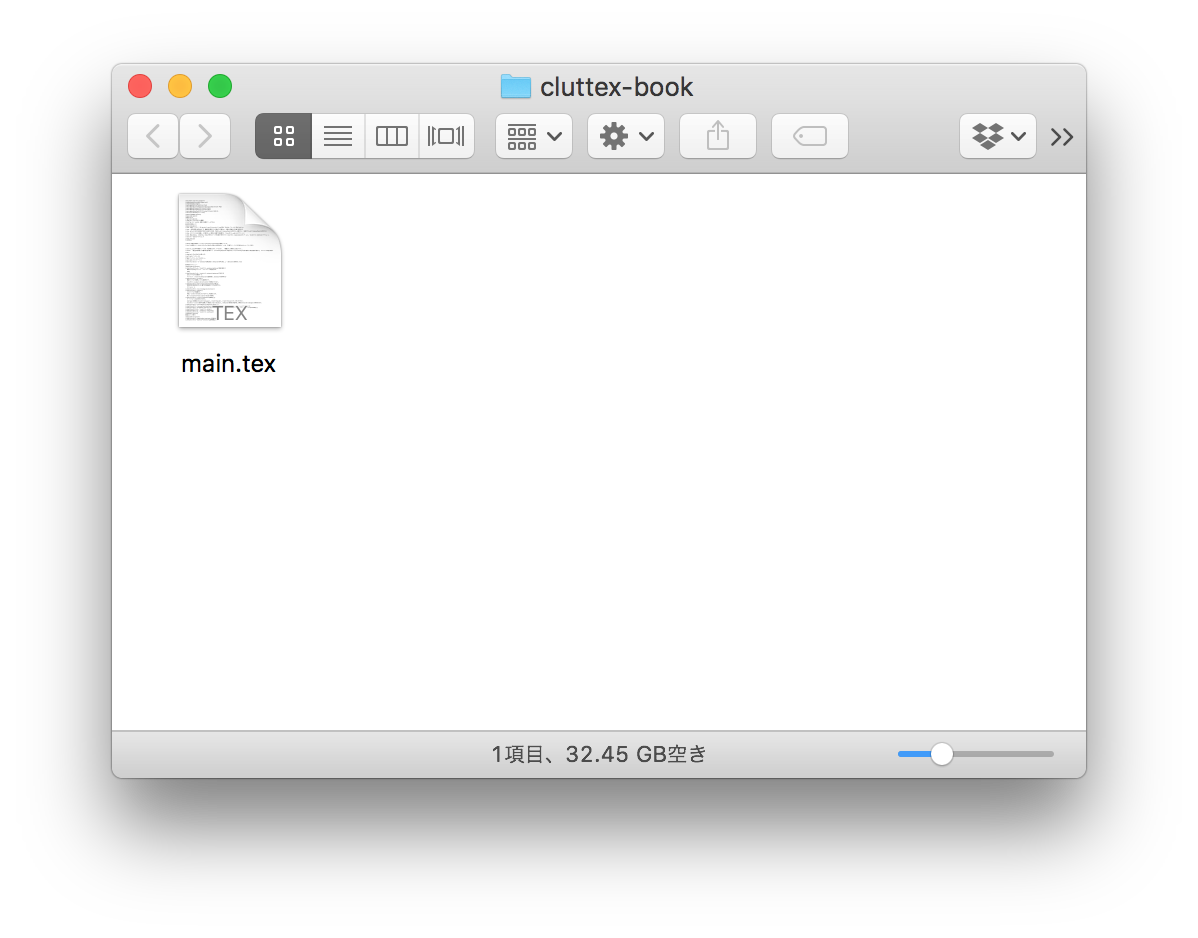
\includegraphics[height=0.6\paperheight]{latex-before.png}\\
    \texttt{\$ lualatex main.tex}
  \end{block}
\end{frame}
\begin{frame}[plain]
  \begin{block}{処理後}
    \centering
    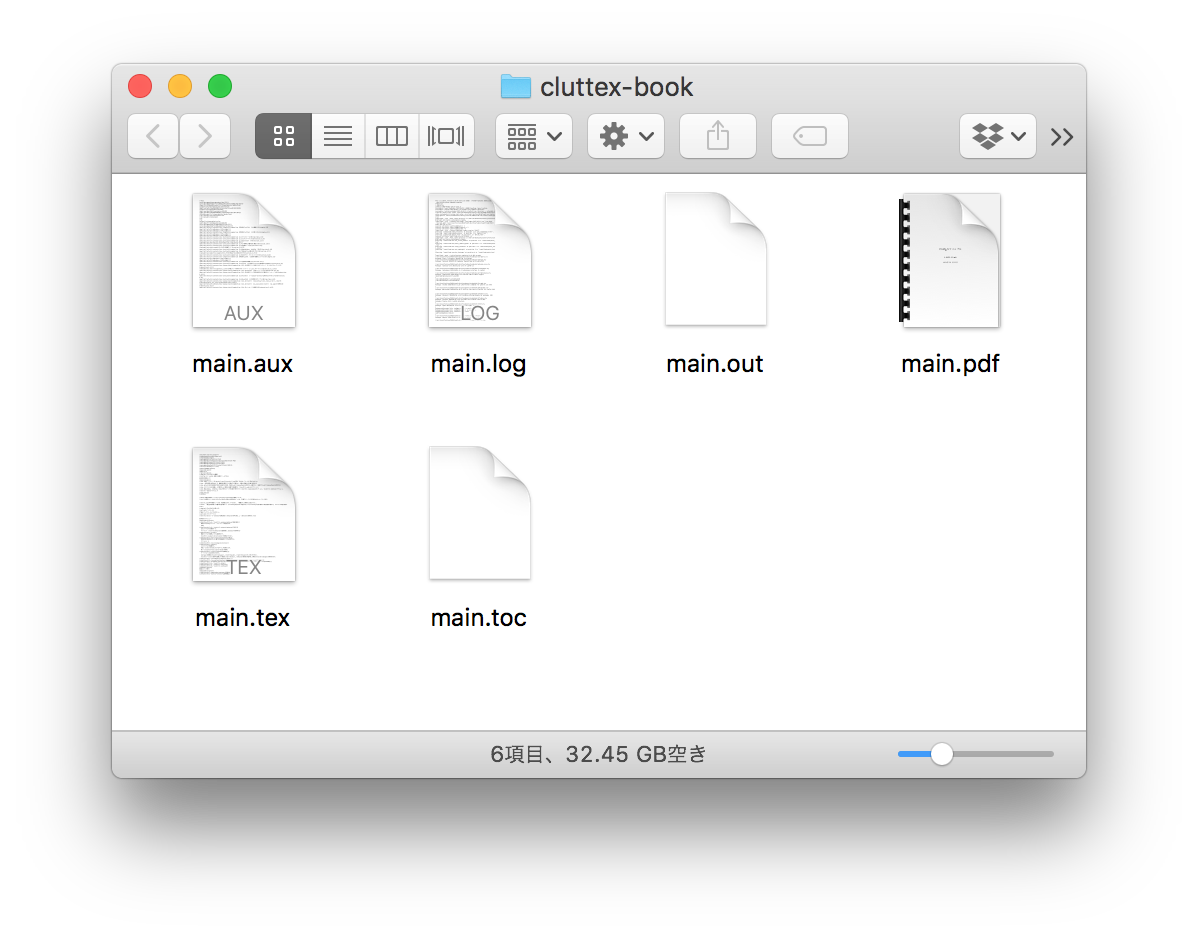
\includegraphics[height=0.6\paperheight]{latex-after.png}\\
    \LARGE ごちゃごちゃ・・・
  \end{block}
\end{frame}
\begin{frame}\frametitle{\LaTeX 処理の問題点}
  手元で処理させる(1.から3.)場合、
  \begin{block}{問題点}
    \begin{center}
      \LARGE \texttt{.aux}や\texttt{.log}等の「余計な」ファイルができる\\
    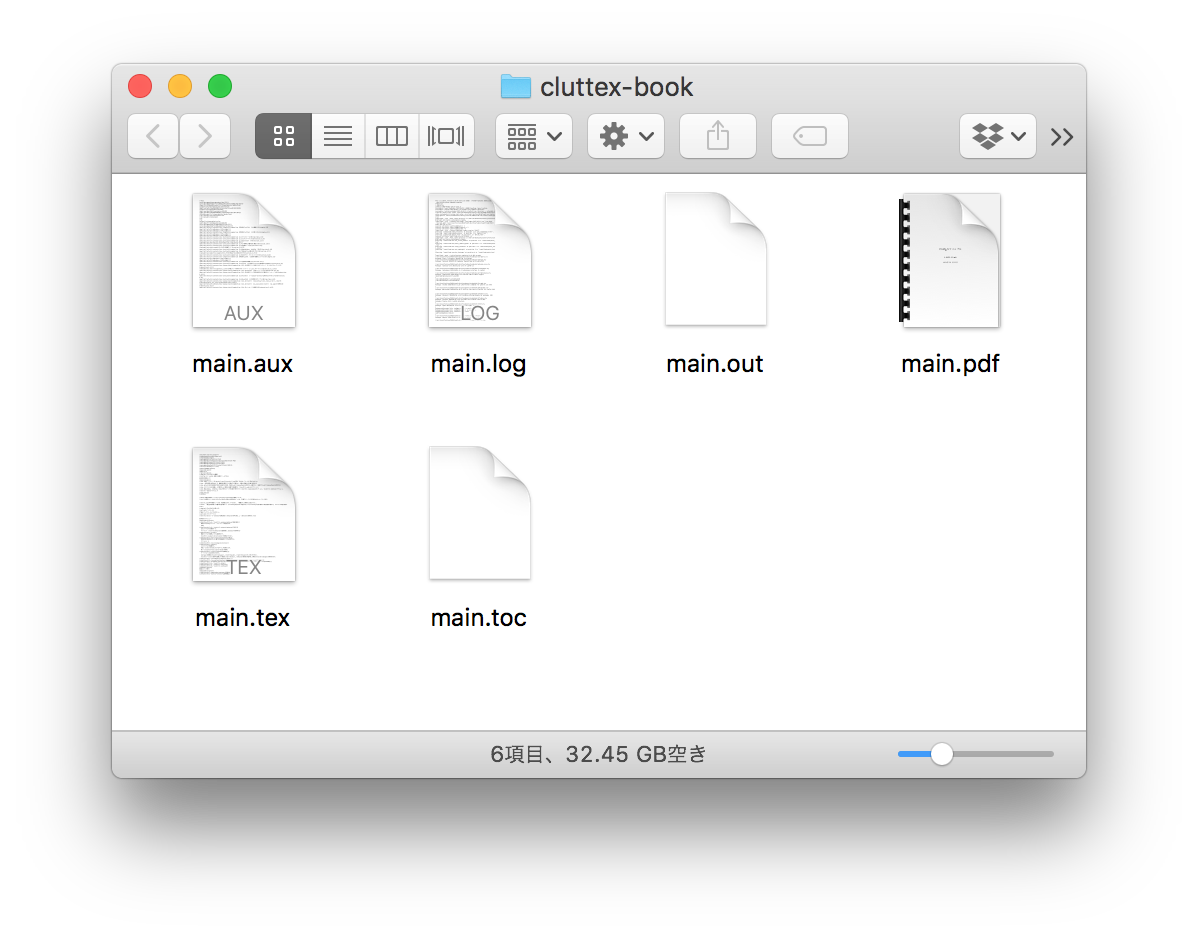
\includegraphics[height=0.5\paperheight]{latex-after.png}
    \end{center}
  \end{block}
\end{frame}
\begin{frame}\frametitle{Clut\TeX の紹介}
  \begin{block}{なにこれ}
    \LaTeX 処理自動化ツール
  \end{block}

  \begin{block}{特徴(主な機能)}
    \begin{itemize}
    \item {\bfseries 余計なファイルを作らない}
    \item 必要に応じて\LaTeX{}処理を複数回行い、相互参照とかを正しくしてくれる
    \item p\TeX{}系でも一発でPDFを生成できる(\texttt{dvipdfmx}を呼び出してくれる)
    \item MakeIndexや\BibTeX と連携できる
    \item 入力ファイルが変化したら自動で再処理できる(監視モード)
    \end{itemize}
  \end{block}

  \begin{block}{作者}
    私(荒田)
  \end{block}
\end{frame}
\begin{frame}[plain]
  \begin{block}{処理前(Clut\TeX{}利用)}
    \centering
    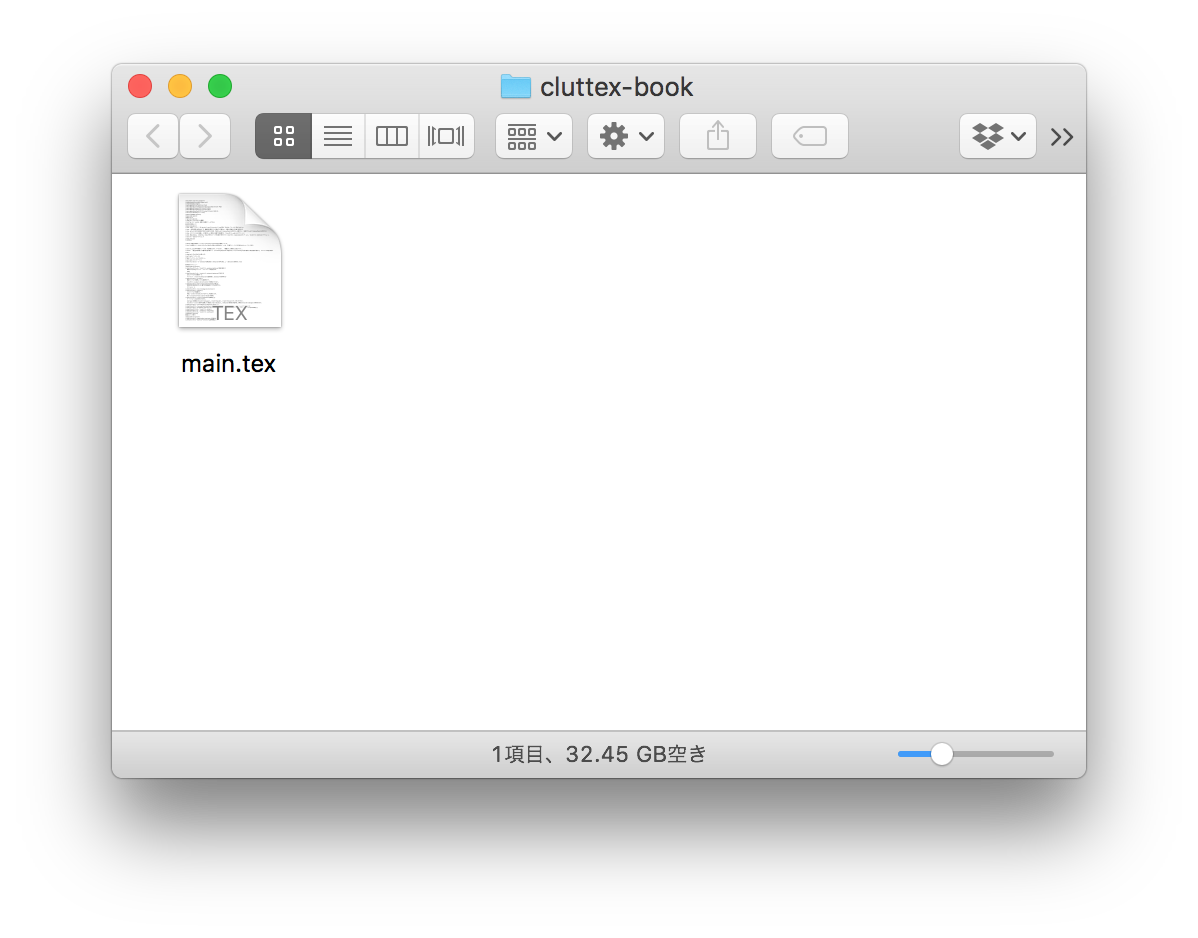
\includegraphics[height=0.6\paperheight]{latex-before.png}\\
    \texttt{\$ cluttex -e lualatex main.tex}\\
    または \texttt{\$ cllualatex main.tex}
  \end{block}
\end{frame}
\begin{frame}[plain]
  \begin{block}{処理後(Clut\TeX{}利用)}
    \centering
    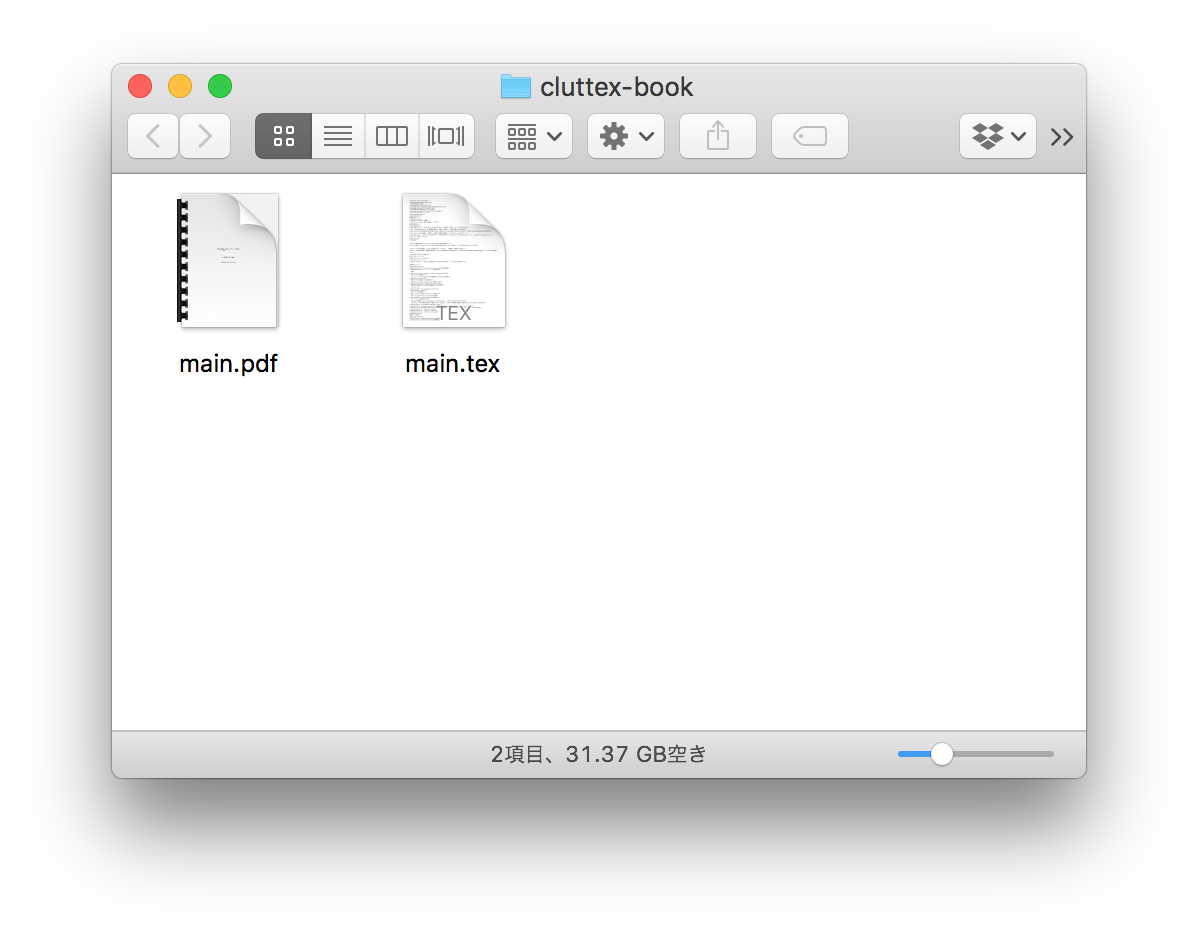
\includegraphics[height=0.6\paperheight]{latex-after-cluttex.png}\\
    \LARGE すっきり!!!
  \end{block}
\end{frame}
\begin{frame}\frametitle{インストール方法}
  \begin{block}{\TeX{} Live}
    今朝収録されました!!!\\
    \texttt{\$ tlmgr update --all}でインストールされるはずです!
  \end{block}

  \begin{block}{手動}
    開発中のバージョンを使いたい人は、
    \begin{enumerate}
    \item \url{https://github.com/minoki/cluttex/releases} を開く
    \item \texttt{.zip}か\texttt{.tar.gz}をダウンロード、展開
    \item \texttt{bin/cluttex} か \texttt{bin/cluttex.bat} を適切な場所にコピー
    \end{enumerate}
  \end{block}
\end{frame}
\begin{frame}\frametitle{今後}
  \begin{block}{機能追加}
    \begin{itemize}
    \item ビューワーの起動
    \item 設定のカスタマイズ(ビューワー、色づけなど)
    \item \TeX worksや\TeX Shopからも使えるようにしたい
    \end{itemize}
  \end{block}

  \begin{block}{普及}
    \begin{itemize}
    \item 使い方の解説記事を書く(英語と日本語)
    \item マニュアルを書く(英語と日本語)
    \item \texttt{latexmk}に替わる選択肢として認知させていきたい
    \end{itemize}
  \end{block}

  \begin{center}
    \LARGE 乞うご期待!
  \end{center}
\end{frame}
\begin{frame}\frametitle{リンク}
  \begin{description}
  \item[GitHub] \url{https://github.com/minoki/cluttex}
  \item[ブログ記事] \url{https://blog.miz-ar.info/2016/12/cluttex/}
  \item[CTAN] \url{https://www.ctan.org/pkg/cluttex}
  \end{description}
\end{frame}
\end{document}
